\documentclass[11pt]{article}

\usepackage[a4paper,margin=25mm]{geometry}
\usepackage{amsmath,amssymb}
\usepackage{booktabs}
\usepackage{graphicx}
\usepackage{microtype}
\usepackage[numbers,sort&compress]{natbib}
\usepackage[hidelinks]{hyperref}

\graphicspath{{figures/}}

\title{TopoDialogue: A Reproducible Instrument for Distinguishing\
Recurrent, Progressive, and Escaping Semantic Trajectories}
\author{Ryoko Sakakibara\\Independent Researcher}
\date{16 August 2026}

\newcommand{\system}{\textsc{TopoDialogue}}
\newcommand{\code}[1]{\texttt{#1}}

\begin{document}
\maketitle

\begin{abstract}
Long human--AI dialogues can return to a similar semantic region without
repeating the same words. A return may simply close a loop, add features and
abstraction, or precede a move into a new region. We present \system{}, a
provenance-aware research instrument for making these distinctions inspectable
and reproducible. The Phase-1 implementation represents turns as a
time-indexed three-dimensional display trajectory, computes recurrence with a
declared feature-set rule, records whether a feature first appeared in a user
or assistant turn, and assigns one of four operational classes: closed loop,
spiral revisit, escape, or open trajectory. The implementation also reports
the input hash, algorithm version, projection seed, axis definitions, and
warnings for known display artefacts. We evaluate the method on six authored
synthetic cases with known structures and run the same manifest through Python
and JavaScript implementations. All twelve declared class and recurrence-source
outputs agree. This is specification conformance, not accuracy on natural
conversation. The result is a reproducible measurement instrument and a set of
testable boundaries, not a psychological, clinical, or topological claim.
\end{abstract}

\section{Introduction}

A dialogue transcript is a sequence, but a sequence alone does not show whether
a later turn returns to an earlier meaning, extends that meaning, or leaves it.
Conversation-dynamics work has shown that interactional movement can complement
the facts and opinions expressed in a transcript \citep{hua2024dynamics}.
Embedding-based work has likewise represented conversational movement as a
trajectory through a high-dimensional space \citep{fischer2024trajectories}.
These precedents motivate a narrower software question: can the recurrence and
change of a single dialogue be represented in a way that another implementation
can reproduce and audit?

The question is important because a visually persuasive curve is easy to
over-interpret. A helix may be caused by a monotonic time coordinate. A loop
may join two speaker-specific branches. A semantic return may be missed when
the input is reduced to lexical overlap. Conversely, a feature annotation can
make a constructed example appear more conclusive than it is. A useful first
paper must therefore define the axes, state the recurrence rule, separate
measurement from rendering, and report failure cases before presenting a
natural-data result.

\system{} is the Phase-1 operationalisation of a broader TopoDialogue design
programme concerned with relational structure, recurrence, provenance,
embodiment, privacy, and control over rendering, introduced in an earlier
concept-and-instrument paper \citep{sakakibara2026topodialogue}. The present
paper implements only the falsifiable core. It makes five contributions:

\begin{enumerate}
  \item a deterministic, versioned input and co-ordinate specification;
  \item operational definitions of revisit, progress, closed loop, spiral
        revisit, escape, and open trajectory;
  \item separate first-occurrence provenance for user- and assistant-originated
        features;
  \item a six-case synthetic conformance suite shared by Python and JavaScript;
        and
  \item an explicit artefact and limitation report that prevents the displayed
        silhouette from being treated as evidence by itself.
\end{enumerate}

The paper does not claim that the instrument detects a person's mental state,
measures therapeutic progress, identifies a mathematical topological invariant,
or improves a conversation. In particular, the name ``TopoDialogue'' is design
provenance. Version 1 computes no persistent homology, Betti number, or other
topological invariant. A separate import or browser-export tool may supply a
conversation file, but export completeness is an acquisition problem outside
the present classifier evaluation.

\section{Positioning and claim boundary}

Research on dialogue dynamics provides a reason to inspect the route through a
conversation rather than only its final state. Hua et al. construct summaries
of interactional dynamics and evaluate them in a downstream forecasting task
\citep{hua2024dynamics}. Fischer and Ram map dyadic conversations into a
high-dimensional space and quantify topical flow and alignment
\citep{fischer2024trajectories}. \system{} shares the interest in movement but
does not infer personality, affect, toxicity, or interpersonal outcome.

Semantic-space planning methods model transitions in order to select future
responses \citep{chen2025scope}. \system{} is retrospective: it does not plan,
generate, or recommend a response. Work on attractor cycles in successive LLM
paraphrasing motivates careful recurrence language \citep{wang2025attractor},
but does not show that ordinary human--LLM dialogues have the same dynamics.
Similarly, simulated multi-turn task results motivate inspection of path
dependence \citep{laban2025lost}; they do not validate the classifier here.

Topological data analysis is an established and developing direction in NLP
\citep{uchendu2026tda}. The present instrument is deliberately weaker: it is a
feature-based geometric display with operational labels. ``Loop'', ``spiral'',
and ``escape'' name finite rules below, not geometric invariants or conclusions
about a person.

\section{Method}

\subsection{Input contract and provenance}

Let a dialogue be $D=(u_1,\ldots,u_T)$. Each turn has a stable identifier, a
speaker in \{user, assistant, system\}, text, and optional structured
annotations. The analyser chooses features in this priority order:

\begin{enumerate}
  \item explicit semantic-node keys, with optional confidence and abstraction;
  \item structured fields such as frame, operator, state, and topic; or
  \item a declared lexical fallback consisting of case-folded words and
        character trigrams.
\end{enumerate}

The selected feature set for turn $t$ is $F_t$. The fallback is deterministic,
but it is not an embedding and cannot reliably identify paraphrase. The report
records the source used for every point and emits a warning when lexical
features are used. For each feature $f$, $o(f)$ is the speaker of the first turn
that contains $f$. New features at turn $t$ are
\begin{equation}
N_t=F_t\setminus\bigcup_{i<t}F_i.
\end{equation}
The counts of user- and assistant-originated novelty are obtained by grouping
$N_t$ by $o(f)$. This records first appearance; it is not a causal attribution
and does not resolve quotation, shared authorship, or anticipation.

\subsection{Coordinates and reproducibility}

Each feature is mapped to three signed hash components using a seeded,
deterministic projection. The feature values are averaged within a turn,
mean-centred over the dialogue, and scaled to $[-52,52]$. The first two
components are the displayed semantic co-ordinates. The default seed is 1729
and is recorded in the report. The input is canonicalised and hashed with
SHA-256; the algorithm version is \code{trajectory-v1}.

The third displayed co-ordinate is selectable:

\begin{description}
  \item[Time] maps turn order linearly to $[-50,50]$. It is monotonic by
        construction and cannot be read as progress.
  \item[Revisit count] maps cumulative visits to an identical feature
        signature to $[-50,50]$.
  \item[Abstraction] maps an explicit annotation, or a declared node-type
        heuristic, from $[0,1]$ to $[-50,50]$. It is not psychological depth.
  \item[Alternative component] uses the third hash component for a projection
        comparison rather than an interpretable axis.
\end{description}

The implementation repeats the semantic projection with seed $1729+104729$.
It reports the Pearson correlation of pairwise distances, clipped to $[0,1]$,
as a projection-stability diagnostic. A value below 0.65 produces a warning.
This two-seed diagnostic does not establish geometric robustness.

\subsection{Recurrence, progress, and LoopScore}

For turn $t$, the analyser searches at most 200 earlier turns and excludes the
immediately preceding turn. Similarity to candidate anchor $j$ is
\begin{equation}
s(t,j)=\frac{|F_t\cap F_j|}{|F_t\cup F_j|}.
\end{equation}
The best eligible anchor is $j_t$. A turn is a revisit when
$s(t,j_t)\geq0.5$. The minimum turn gap is two.

Let $a_t\in[0,1]$ be the operational abstraction value. On a revisit,
\begin{equation}
p_t=\min\left(1,0.7\frac{|N_t|}{\max(1,|F_t|)}+
0.3\max(0,a_t-a_{j_t})\right).
\end{equation}
For the revisit set $R$, the report gives mean similarity $\bar{s}$, mean
progress $\bar{p}$, and
\begin{equation}
\mathrm{LoopScore}=\operatorname{clip}_{[0,1]}\bigl(\bar{s}(1-\bar{p})\bigr).
\end{equation}
LoopScore is a descriptive software quantity. It is not a calibrated measure
of psychological state, conversational quality, or clinical risk.

\subsection{Operational classes}

Classification uses the following priority order:

\begin{enumerate}
  \item fewer than three turns: \emph{insufficient data};
  \item no revisits: \emph{open trajectory};
  \item an escape event: \emph{escape};
  \item mean revisit progress or mean positive abstraction gain at least 0.2:
        \emph{spiral revisit};
  \item otherwise: \emph{closed loop}.
\end{enumerate}

After a revisit, Escape@5 is true if, within the next five turns, a user turn
has best similarity below $0.5\times0.55=0.275$, introduces at least one new
feature, and is followed by no further revisit in that finite window. The
priority rule explains why an escape case may have LoopScore 1: the score
describes the preceding recurrent region, while the class records the later
transition. Recurrence source is the majority speaker of revisit turns; ties
are \emph{mixed}, and no revisits are \emph{none}.

\section{Synthetic validation}

\subsection{Design and protocol}

The validation manifest contains six authored six-turn fixtures with explicit
node keys and abstraction values. The cases are exact loop, spiral revisit,
open trajectory, assistant-induced loop, spiral escape, and speaker drift. The
expected class and recurrence source are declared before the runner executes.
The Python reference implementation and the JavaScript visualiser consume the
same fixture manifest. Repeated runs compare the complete report under one
seed; a second seed is used to test that geometry may change while operational
metrics remain stable.

\subsection{Results}

Table~\ref{tab:synthetic} reports the regenerated Python result for
\code{trajectory-v1}, seed 1729. Both implementations match all twelve
declared outputs: six classes and six recurrence-source labels. This is exact
conformance on constructed examples, not $100\%$ accuracy in a sampled
population.

\begin{table*}[t]
\centering
\small
\caption{Synthetic Phase-1 results. $r$ is revisit rate, $\bar{s}$ mean
revisit similarity, $\bar{p}$ mean progress on revisit, $L$ LoopScore, $E$
Escape@5, and $\rho$ projection stability.}
\label{tab:synthetic}
\begin{tabular}{llrrrrrr}
\toprule
Case & Class/source & $r$ & $\bar{s}$ & $\bar{p}$ & $L$ & $E$ & $\rho$ \\
\midrule
Exact loop & closed/mixed & .666667 & 1.000000 & .000000 & 1.000000 & No & 1.000000 \\
Spiral revisit & spiral/mixed & .666667 & .583333 & .243333 & .441389 & No & .939956 \\
Open trajectory & open/none & .000000 & .000000 & .000000 & .000000 & No & .442795 \\
Assistant loop & closed/assistant & .333333 & 1.000000 & .000000 & 1.000000 & No & .434584 \\
Spiral escape & escape/mixed & .333333 & 1.000000 & .000000 & 1.000000 & Yes & .824146 \\
Speaker drift & closed/mixed & .666667 & 1.000000 & .000000 & 1.000000 & No & 1.000000 \\
\bottomrule
\end{tabular}
\end{table*}

The spiral-revisit case differs from the exact loop because revisits add
features and increase the supplied abstraction value. The assistant-induced
case records assistant recurrence separately from user recurrence. The open
and assistant-induced cases trigger projection warnings because $\rho<0.65$.
The escape fixture demonstrates why class and score must be reported together.

\begin{figure*}[t]
\centering
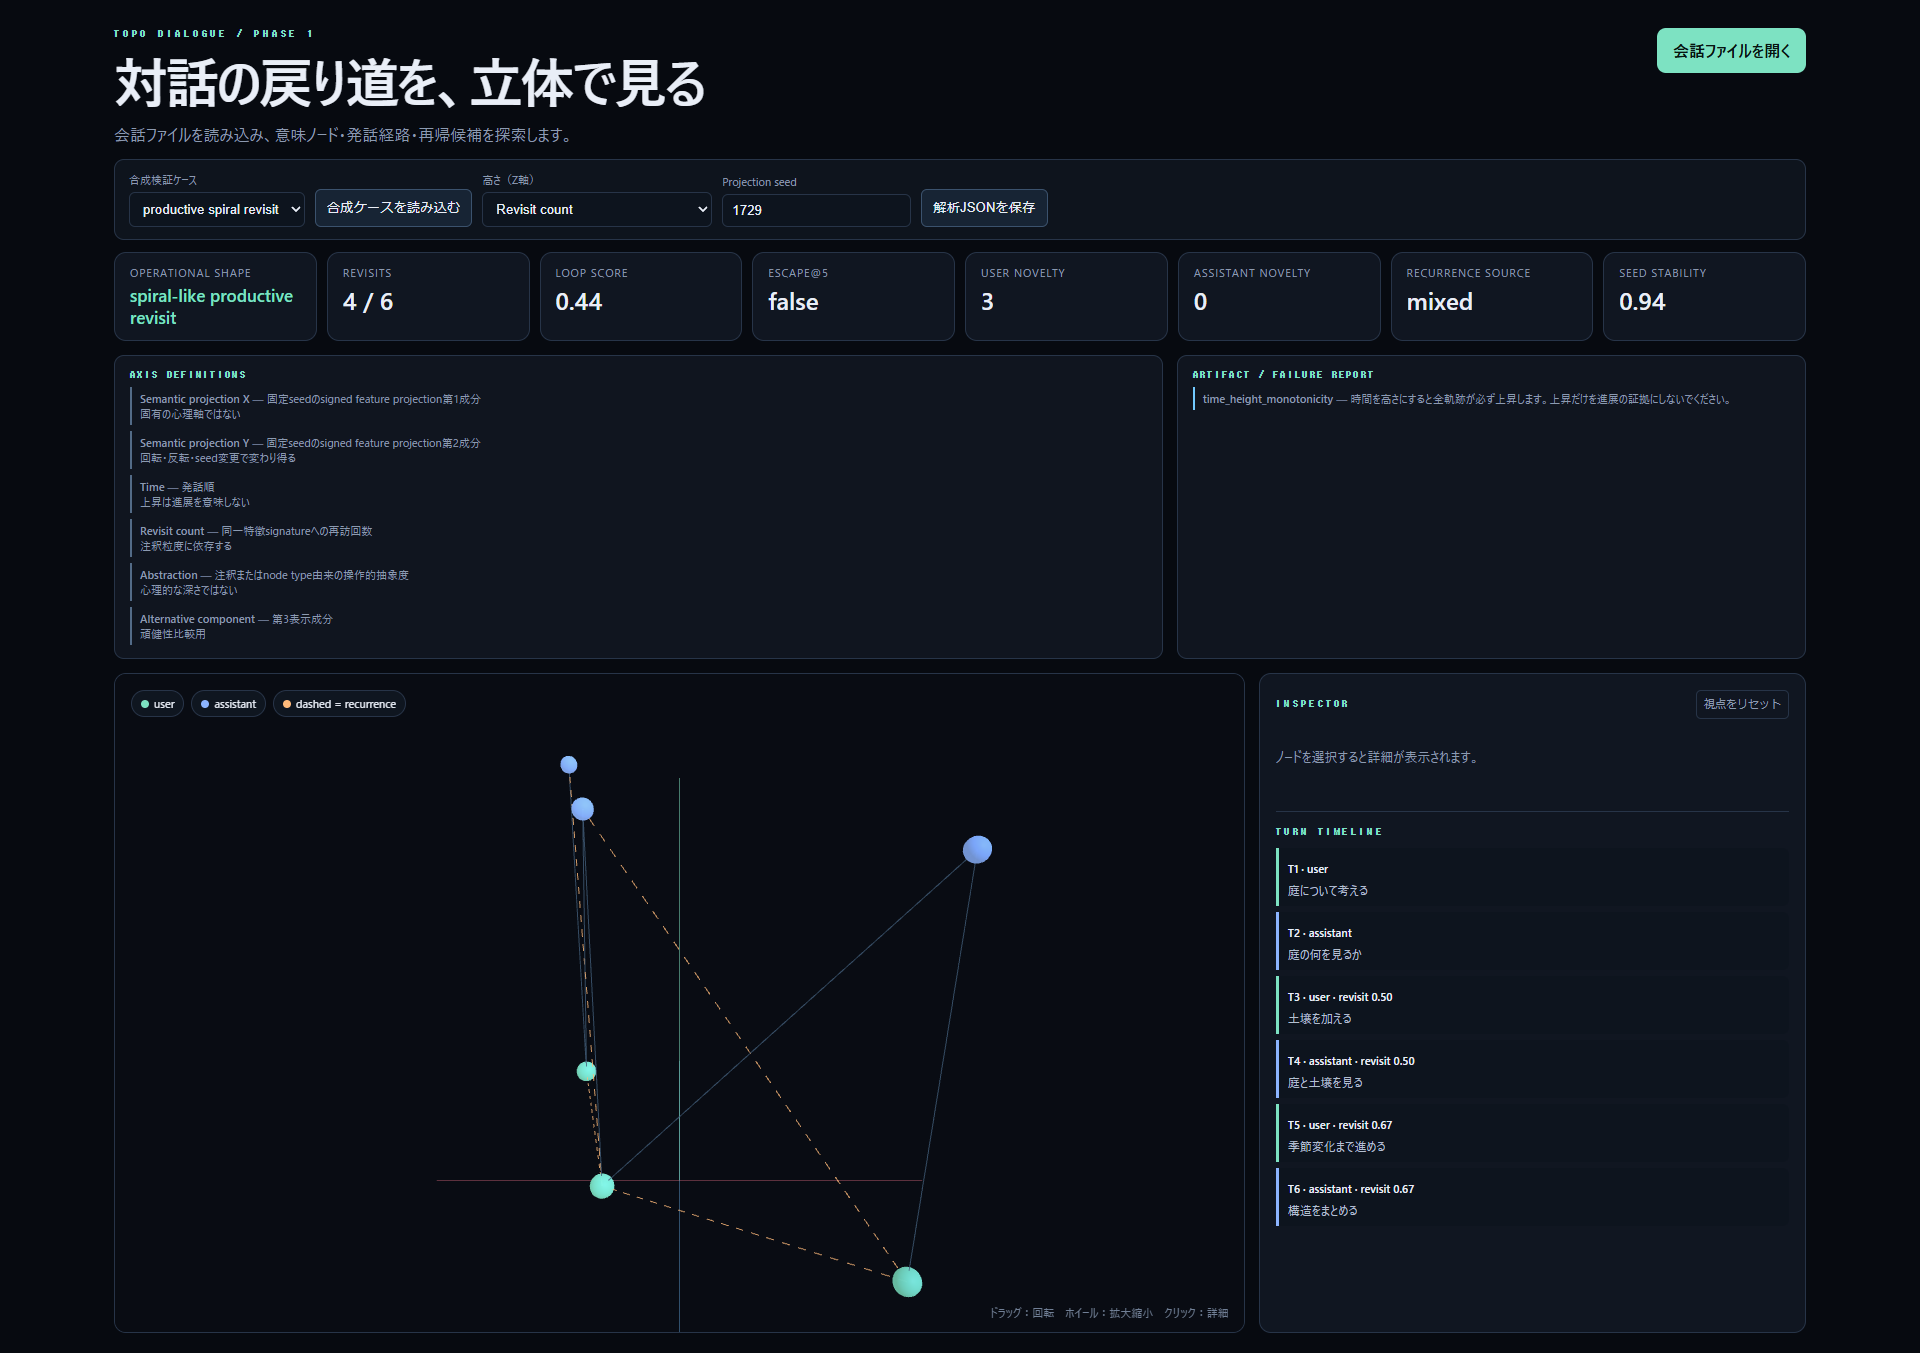
\includegraphics[width=.48\textwidth]{fig01-spiral-revisit.png}\hfill
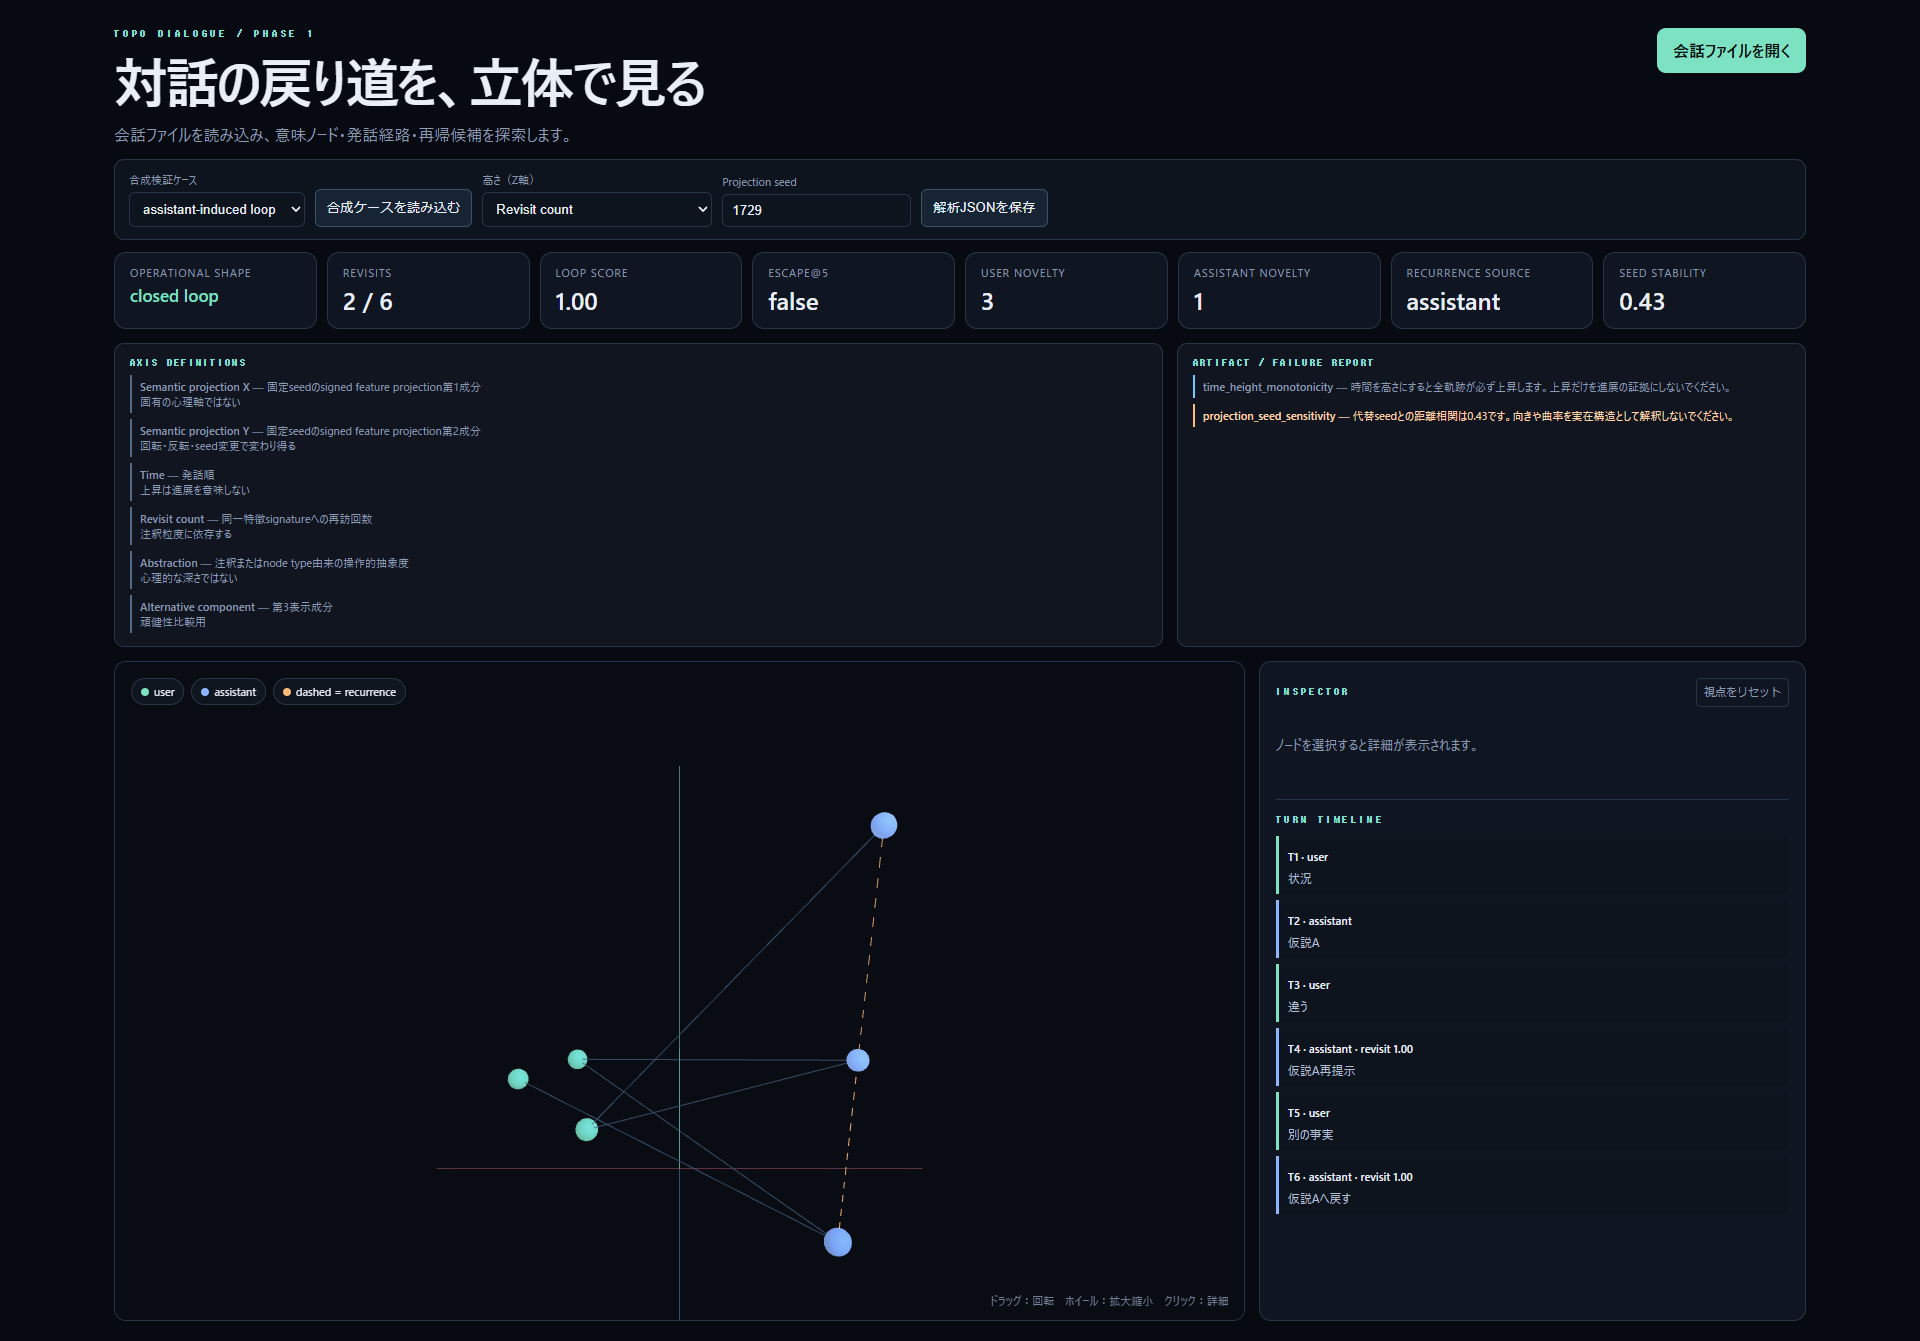
\includegraphics[width=.48\textwidth]{fig02-assistant-induced-loop.png}
\caption{Two synthetic trajectories. Shape labels come from feature-based
rules, not from visual curve recognition.}
\label{fig:synthetic-first}
\end{figure*}

\begin{figure*}[t]
\centering
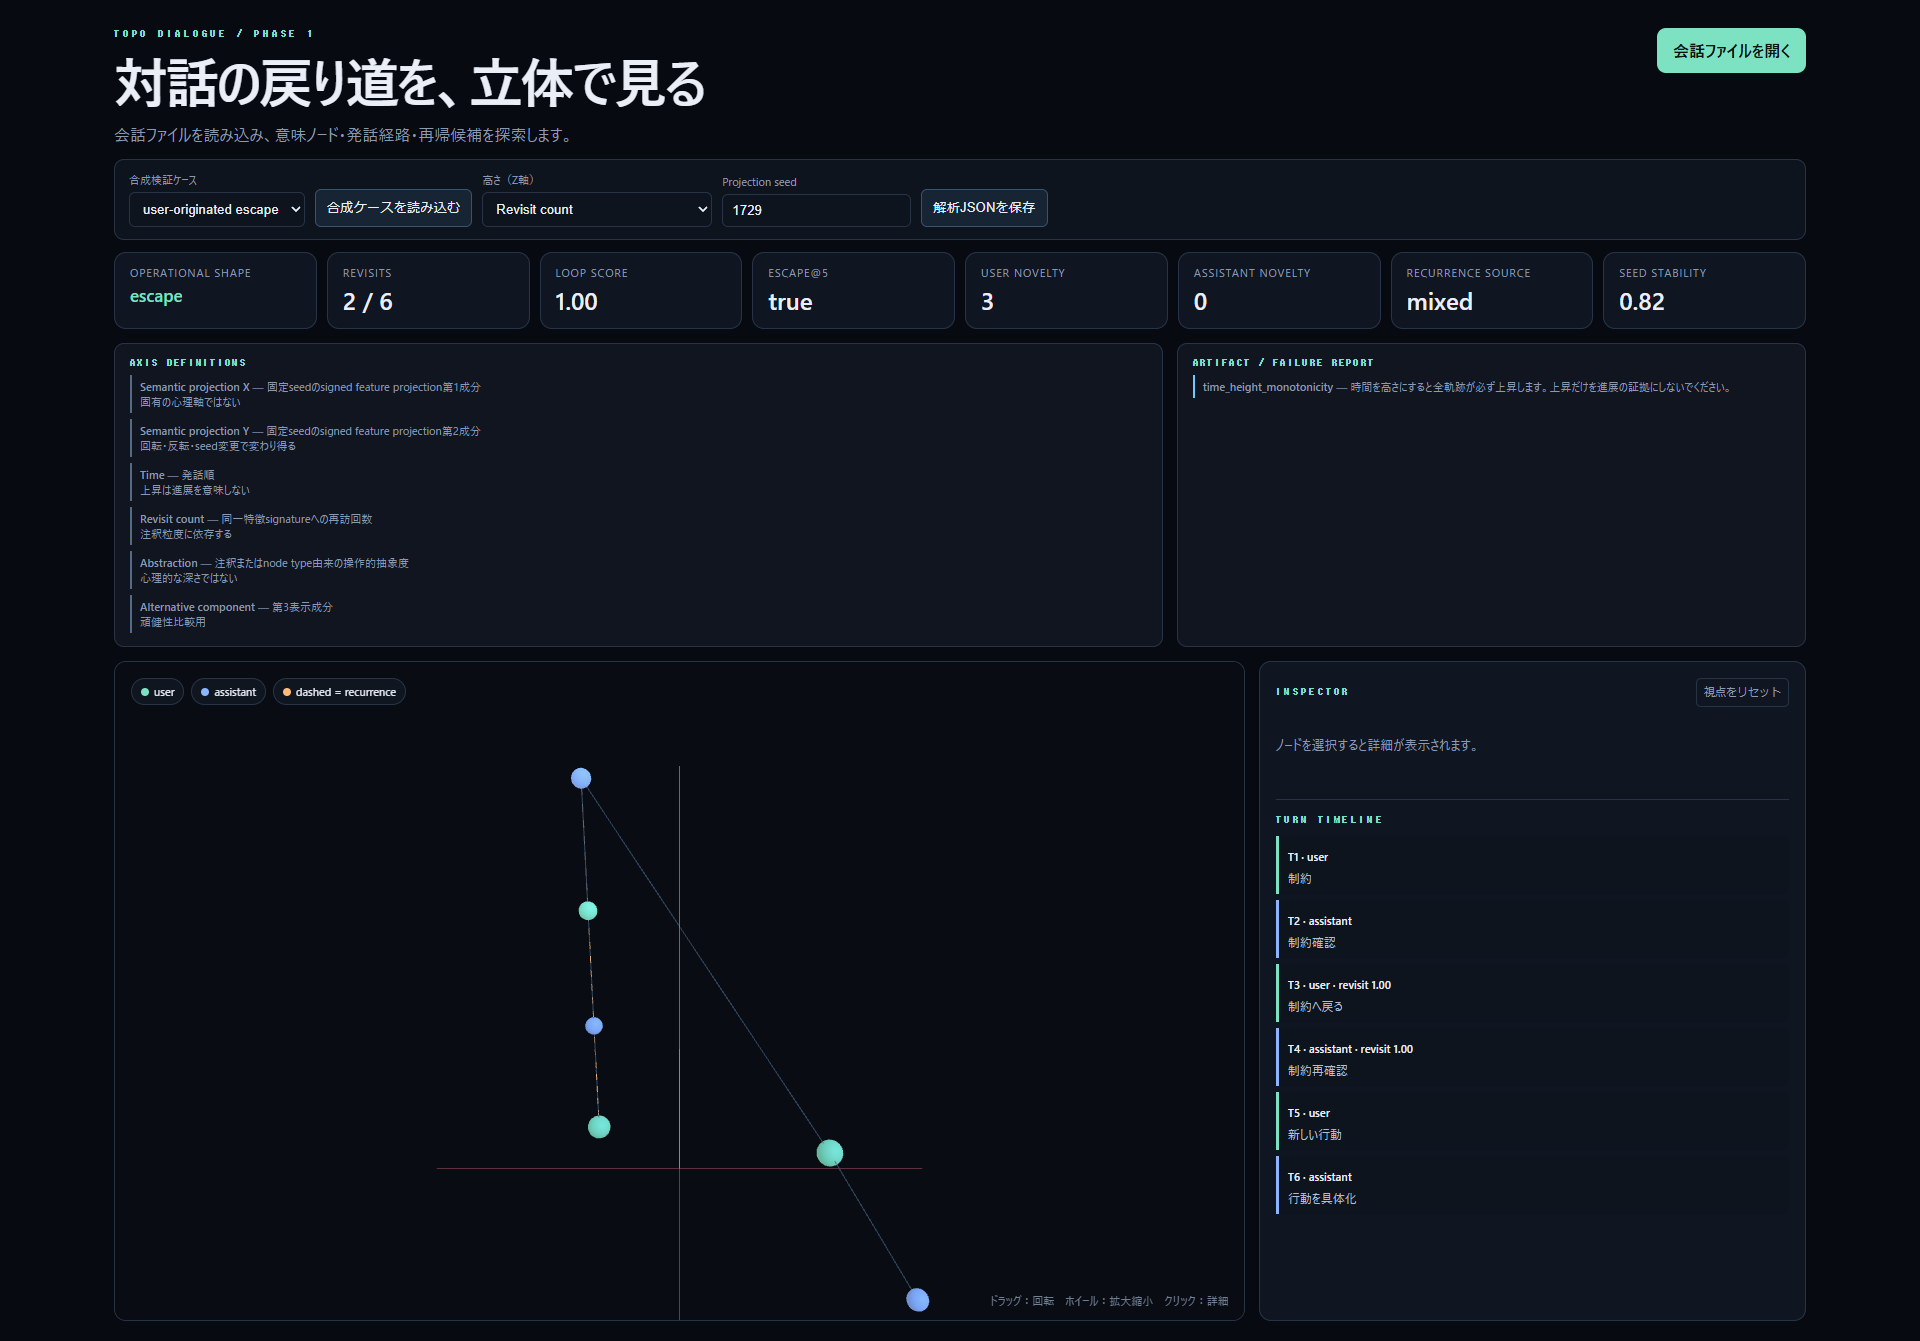
\includegraphics[width=.48\textwidth]{fig03-user-originated-escape.png}\hfill
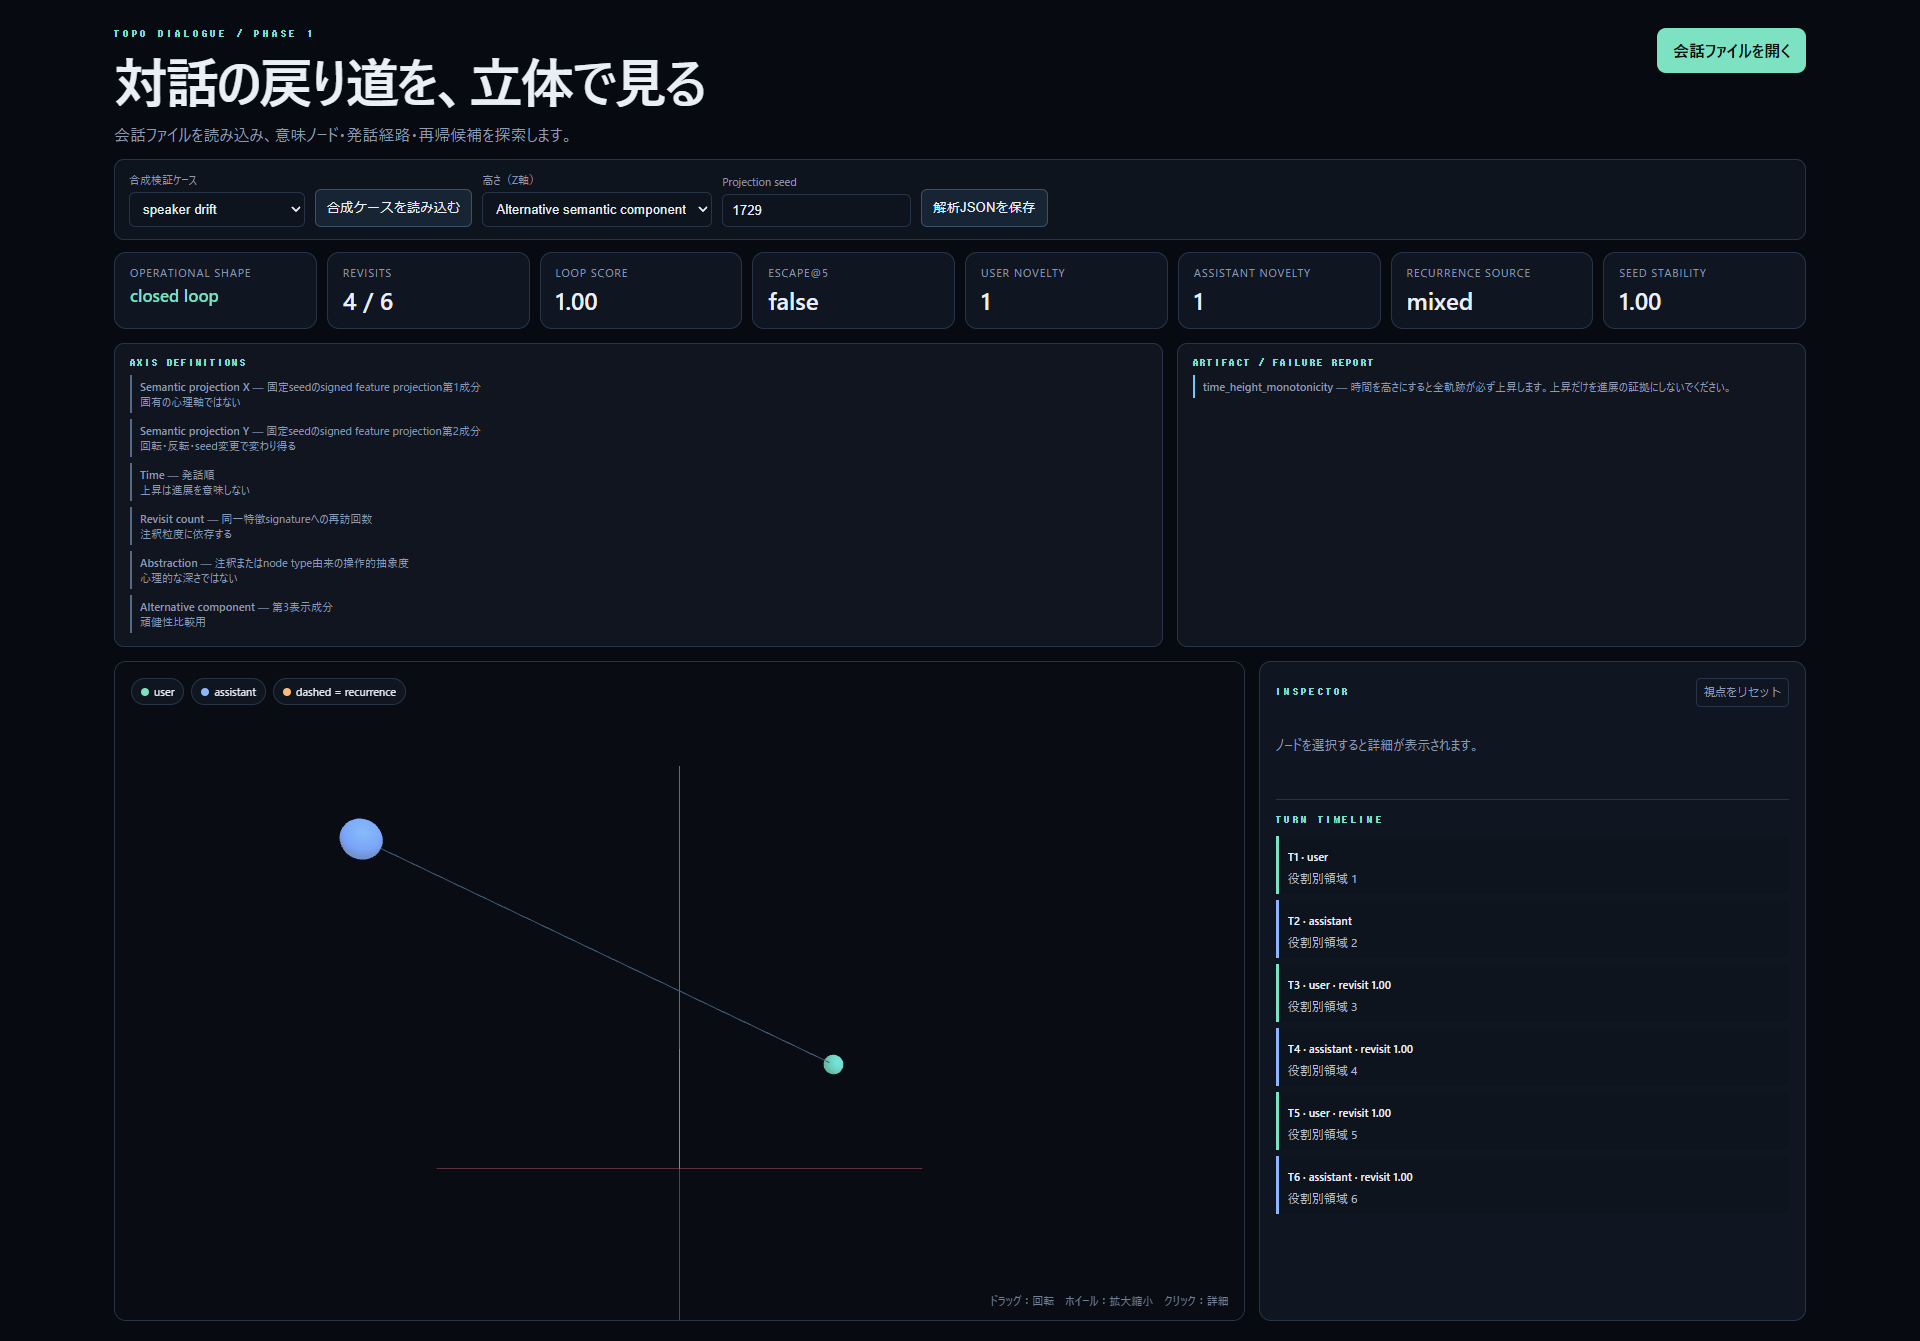
\includegraphics[width=.48\textwidth]{fig04-speaker-drift-artifact.png}
\caption{A user-originated escape and a speaker-drift stress case. The latter
shows why a striking silhouette is not evidence of one shared semantic cycle.}
\label{fig:synthetic-second}
\end{figure*}

\section{Artefacts, privacy, and failure analysis}

\paragraph{Monotonic time.}
Time height makes every path rise. A helix-like display can therefore be a
rendering consequence. The classifier never uses upward motion as progress and
the report emits a monotonic-time warning.

\paragraph{Lexical fallback and annotation dependence.}
Unannotated input uses words and character trigrams. It is reproducible but
misses semantic paraphrase and may overstate orthographic overlap. Explicit
node keys make authored fixtures easier than natural text. A natural-data
study must compare lexical, embedding, and human-annotation pipelines rather
than merge their outputs.

\paragraph{Projection and speaker drift.}
Hash projections do not guarantee neighbourhood fidelity. Two speaker-specific
branches can be joined by one polyline and appear to be a single cycle. Point
provenance, speaker-aware recurrence source, and the stability warning expose
part of this risk, but they do not solve it.

\paragraph{Acquisition boundary.}
The analyser accepts a structured conversation file as input. It does not prove
that a browser, desktop client, or command-line exporter captured every turn.
Missing turns, duplicated turns, and UI labels must be audited before trajectory
analysis. The input hash makes the analysed file identifiable, not complete.

\paragraph{Privacy and intended use.}
Dialogue logs can contain intimate or identifying information. Local execution
does not itself provide consent, access control, retention limits, or safe
publication. Researchers should minimise collection, redact before sharing,
retain provenance, and avoid publishing raw personal conversations. \system{}
is not a clinical, therapeutic, diagnostic, or risk-scoring tool. Its terms
refer only to the finite rules in this paper and must not label a person as
stuck, recovered, insightful, resistant, or healthy.

\section{Limitations and next study}

The evidence has five principal limits. First, six authored cases do not
establish external validity. Secondly, supplied annotations may encode the
expected answer. Thirdly, fixed hash projections are display devices rather
than learned semantic representations. Fourthly, thresholds are design
constants, not estimates from labelled data. Fifthly, first appearance cannot
resolve shared authorship or causal influence.

The next study should preregister an annotation protocol and use held-out
natural dialogues with multiple annotators. It should measure agreement for
recurrence, productive revisit, and escape; compare lexical, embedding, and
annotated features; test multiple seeds and projection families; report
class-wise precision, recall, and calibration; and measure provenance errors
separately from shape errors. A blinded ablation should compare the three-
dimensional view with a transcript, similarity matrix, and two-dimensional
timeline. Transformation operators and online effects should be evaluated only
after this measurement layer has been validated.

\section{Conclusion}

\system{} turns a broad proposal about preserving dialogue structure into a
small falsifiable instrument. It defines axes, fixes a reproducibility contract,
distinguishes operational recurrence classes, separates first-occurrence
provenance, and reports ways in which a display can mislead. The six synthetic
cases show that the software implements its declared rules. They do not show
that natural conversations reliably have these forms. The defensible result of
this second draft is methodological: same-region revisits and change within
those revisits can be measured before they are presented as shapes.

\section*{Language and reproducibility note}

The manuscript prose is written in British English. Published titles retain
their original spelling. The code, fixture manifest, tests, figure captures,
and audit are versioned with the project. The preceding design paper is cited
through its public Zenodo DOI. A dedicated archival software release remains
future work; no unavailable identifier is cited.

\bibliographystyle{plainnat}
\bibliography{references}

\end{document}
